\documentclass[12pt]{article}

\usepackage{url}
\usepackage{hyperref}
\usepackage[margin=1in]{geometry}
\usepackage{graphicx}
\usepackage{color}
\usepackage{listings}
\definecolor{ao}{rgb}{0.0, 0.5, 0.0}
\lstset
{ %Formatting for code in appendix
	language=C++,
	numbers=left,
	stepnumber=1,
	showstringspaces=false,
	tabsize=1,
	breaklines=true,
	breakatwhitespace=false,
	keywordstyle=\color{blue},
	stringstyle=\color{red},
	commentstyle=\color{ao},
	morecomment=[l][\color{magenta}]{\#}
}

\newcommand{\forceindent}{\leavevmode{\parindent=1em\indent}}

\begin{document}
	\begin{titlepage}
		\centering
		{\scshape\LARGE Project Summary \par}
		\vspace{1cm}
		{\scshape\Large CS 383\par}
		\vspace{1.5cm}
		{\huge\bfseries Group \#4\par}
		\vspace{2cm}
		{\Large\itshape Trevor Morse\par}
		{\Large\itshape Peter Fetros\par}
		{\Large\itshape Zachary Spence\par}
		{\Large\itshape Adonay Berhe\par}
		{\Large\itshape Matthew Holman\par}
		{\Large\itshape Domanic Welker\par}
		\vfill
		supervised by\par
		Mr. Bruce \textsc{Bolden}
		
		\vfill
	\end{titlepage}
	
	\tableofcontents
	\clearpage
	
	\section{General}
	\subsection{Task}
	\begin{itemize}
		\item Create a new version of the Tower Animator Program.
	\end{itemize}
	\subsection{Design Decisions}
	The first step of this project was to create a design specification. We knew that we needed to mimic the functionality of the existing Tower Animator Program, however, we decided to run with a different UI design. Our goal was to layout an interface that was intuitive to use and provided the necessary functions with ease of access. In order for the program to have a familiar interface, we borrowed ideas from other editing programs. We decided to have two primary sections to the interface:
	\begin{itemize}
		\item A toolbox that provides controls for editing the overall animation.
		\begin{figure}[!htb]
			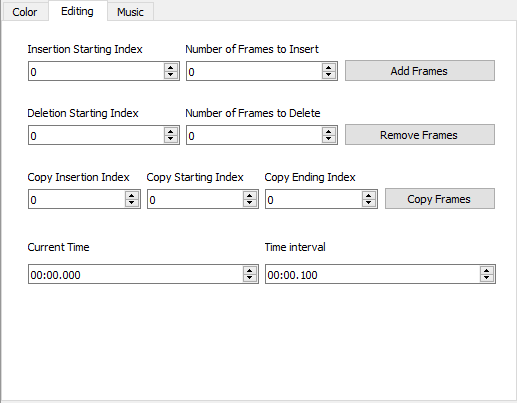
\includegraphics[]{./screenshots/toolbox}
			\caption{Screen shot depicting the toolbox section of the program.}
			\label{fig:toolbox}
		\end{figure}
		\clearpage
		\item An editor that allows for manipulation of individual frames at a time.
		\begin{figure}[!htb]
			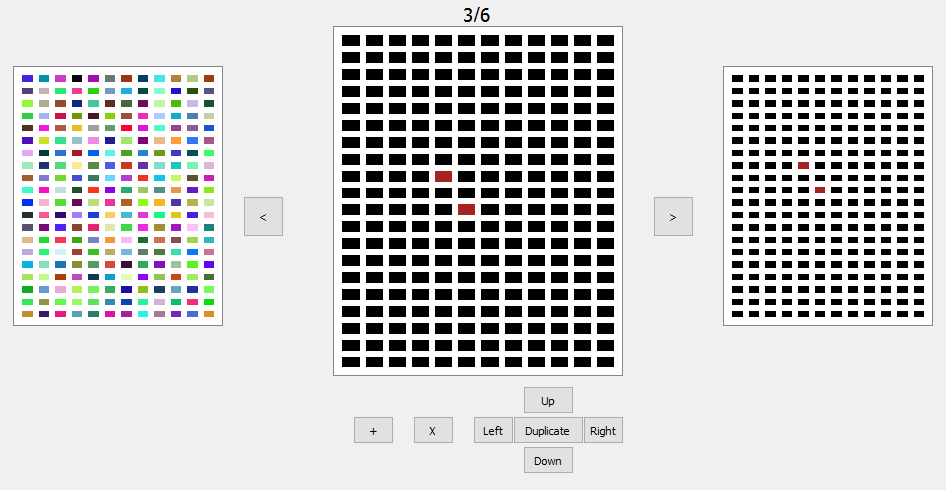
\includegraphics[width=\linewidth]{./screenshots/editor}
			\caption{Screen shot depicting the editor section of the program.}
			\label{fig:editor}
		\end{figure}
	\end{itemize}
	By organizing our program into these two sections, we not only were able to have a solidified design to work with, but we were also able to use the different sections as clear work divisions for the team throughout the project. 
	
	\clearpage
	\section{Development}
	\subsection{Process}
	Throughout most of the project, our team of six split into pairs and divvied up work accordingly. Two members (Peter and Trevor) worked on the back-end code, handling the file I/O and associated data structures. Two more (Matthew and Domanic) worked on the UI for the toolbox section. The remaining two (Adonay and Zachary) worked on the UI for the editor section. This work division remained intact for most of the project, however, in the final couple of weeks, team members previously working on other sections stepped in to help out in certain areas. (For example, Peter and Trevor helped complete the UI and connect the slots for both the editor and toolbox.) 
	\subsection{Issues}
	As with any project, this one was not free of issues. Throughout the development process, our team hit its fair share of bumps and did our best to overcome and continue making progress. The overarching issue we had was inexperience with a software engineering project of this proportions. With the exception of two members, our team was new to product design, version control, and collaborative work. Resolving this issue was an ongoing process and simply requires time and experience.\\
	\\
	Another issue we faced as a team was unfamiliarity with Qt. This primarily surfaced in relation to the UI work. There was some confusion early on about how to create an interface and layout elements appropriately. However, this issue was more or less resolved as members gained more experience and were able to help each other out from their findings.\\
	\\
	We also faced issues of features and/or interfaces not being implemented as expected. This was due to not having spent enough time on our design spec at the beginning and also not enforcing the team's reference of the spec. This could easily be prevented in future projects by solidifying the design details earlier as well as emphasizing the need for the entire team to be making consistence reference back to the spec while working on implementation.
	
	\clearpage
	\section{Remaining Work}
	\subsection{Features}
	Due to the time constraints of the project and the abilities of our team, our project ended with  the core functionality of the program implemented. That being said, there is plenty more that could be added to this project. Our UI is minimalistic and could benefit from some enhancements and cleanup for a more polished interface. Our menu options are very limited and could be expanded to have more file controls as well as more controls for manipulating the animation. We also did not have time to implement additional features such as previewing an animation or inserting pre-defined mini-animations into an overall animation. (For a more detailed listing of additional features, please see Section 5 of our Design Specification.)
	\subsection{Time Estimate}
	Our project had a slow start at the outset as our team familiarized itself with processes and Qt. However, in the last couple of weeks, we started to hit more of a rhythm and made a substantial amount of progress (as compared with the start). We would estimate another 3-4 weeks of work in order to cleanup the UI, round out the menu options, and add features like previewing the animation or inserting pre-defined mini-animations. This estimate assumes continued work at the same pace, i.e. we are still taking other classes and are not able to work on this project full-time. This estimate also does not include adding more advanced features like integrating the music file with the animation creation.
	
	\clearpage
	\section{Overview}
	Overall, despite the bumps faced along the way, this project was successful for the purposes of the class. Our team gained experience working with Git, Qt, and Slack, all of which are tools utilized in real-world software engineering projects. We made mistakes that provided valuable learning experiences, both in terms of teamwork and development. Finally, we were able to complete a program that satisfied the core functionality requirements of the Tower Animator Program.
\end{document}
